%30.10.2024, lecture 4

\section{Properties of Distributions}

\subsection{Entropy Profiles}

For any random variable $\alpha$ on $\{a_1, \ldots, a_n\} $.
Then,
\[
\log n \ge H(\alpha) \ge 0.
\] 
Then, what about entropy in the middle?

\begin{center}
\begin{tabular}{c|c}
	$p_1, \ldots, p_n$ & $H(\alpha)$ \\
	\hline
	$\frac{1}{n}, \ldots \frac{1}{n}$ & $\log n$ \\
	$0, \ldots, 0, 1$ & 0 \\
\end{tabular}
\end{center}

What about $\alpha$ with probabilities $a(\frac{1}{n}, \ldots, \frac{1}{n}) + (1 - a) (0, \ldots, 1)$ for some $a \in [0, 1]$?
Obviously, it is a random variable since it is a combination of two random variables with proper norm.
Now, we need to proof that entropy is a continuous function.
And the entropy is continuous since it is a linear combination of many linear functions.
Hence, we've proved the next theorem.

\begin{theorem}
	For any $h \ge  0$, there exists a distribution $\alpha$ such that $H(\alpha) = h$.
\end{theorem}

Now, what about two variables?
Let's consider entropy profile $(H(\alpha), H(\beta), H(\alpha, \beta))$.
\begin{theorem}
	For any numbers $h_1, h_2, h_{12} \geq 0$, that satisfy the following relations:
	\begin{align*}
		\begin{cases}
			h_{12} \le  h_1 + h_2 \iff t_0 = I(\alpha : \beta) \ge 0 \\
			h_2 \le  h_{12} \iff t_1 = H(\alpha | \beta) \ge 0 \\
			h_1 \le  h_{12} \iff t_1 = H(\beta | \alpha) \ge 0 \\
		\end{cases}
	\end{align*}
\end{theorem}
\begin{proof}
	Let $\xi_0, \xi_1, \xi_2$ be independent random variables with entropies $t_0, t_1, t_2$, respectively.
	Then, $\alpha = (\xi_0, \xi_1)$ and $\beta = (\xi_0, \xi_2)$.
	\begin{align*}
		\begin{cases}
			H(\xi_0) = t_0 = h_1 + h_2 - h_{12} \\
			H(\xi_1) = t_1 = h_{12} - h_2 \\
			H(\xi_2) = t_2 = h_{12} - h_1 \\
		\end{cases}
	\end{align*}
	See \Cref{fig:IMG_8BB43F4ACC89-1}.
	\begin{figure}[htpb]
		\centering
		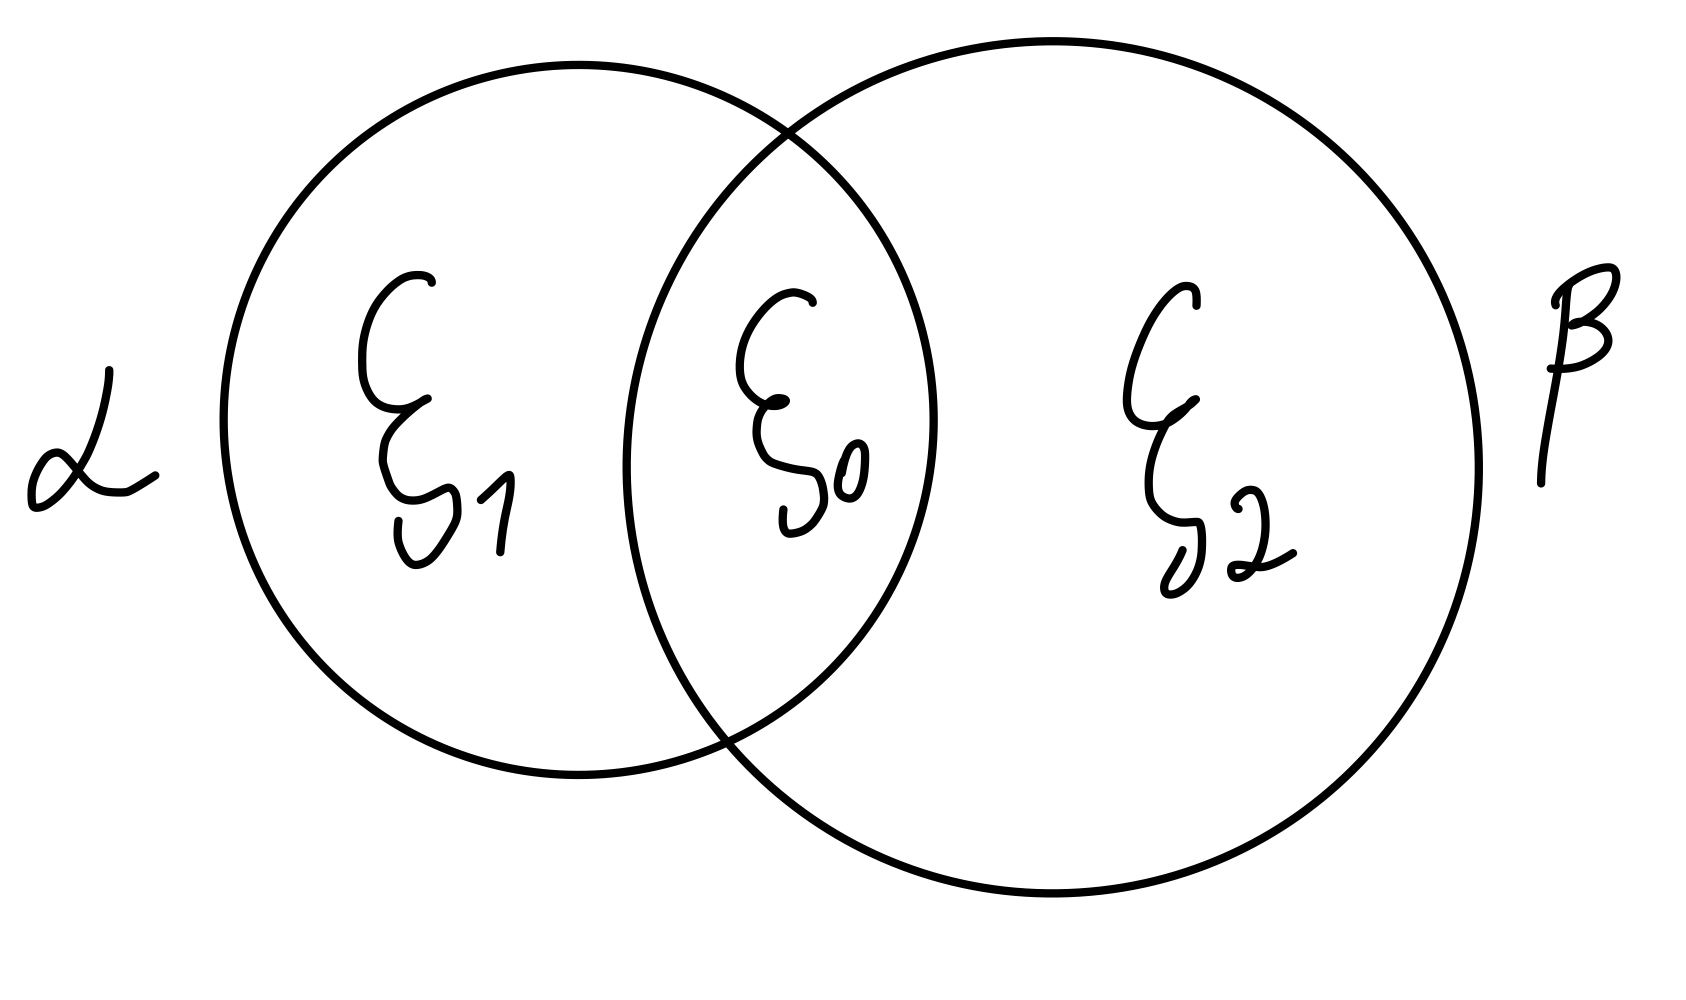
\includegraphics[width=0.3\textwidth]{IMG_8BB43F4ACC89-1}
		\caption{Structure of $\alpha, \beta$.}
		\label{fig:IMG_8BB43F4ACC89-1}
	\end{figure}
\end{proof}

Now, three random variables.
The entropy profile is 
\[(H(\alpha), H(\beta), H(\gamma), H(\alpha, \beta), H(\alpha, \gamma), H(\beta, \gamma), H(\alpha, \beta, \gamma)).\]

For the random varibales $(\alpha, \beta, \gamma)$ we can write 9 independent inequalities.
\begin{align*}
	H(\alpha  \mid  \beta, \gamma) &\ge 0, \quad I(\alpha : \beta) \ge  0, \quad I(\alpha : \beta  \mid  \gamma) \ge  0, \\
	H(\beta  \mid  \alpha, \gamma) &\ge 0, \quad I(\beta : \gamma) \ge  0, \quad I(\beta : \gamma  \mid  \alpha) \ge  0, \\
	H(\gamma  \mid  \beta, \alpha) &\ge 0, \quad I(\alpha : \gamma) \ge  0, \quad I(\gamma : \alpha  \mid  \beta) \ge  0.
\end{align*}
It is clear that you can assign such profile that one of those inequalities is not satisfied.
Our trick does not work because the entropy of $I(\alpha : \beta : \gamma)$ could be negative.
See \Cref{fig:IMG_FFE63C0B5F05-1}.
Entropy profile just encodes values in the circles.

\begin{figure}[htpb]
	\centering
	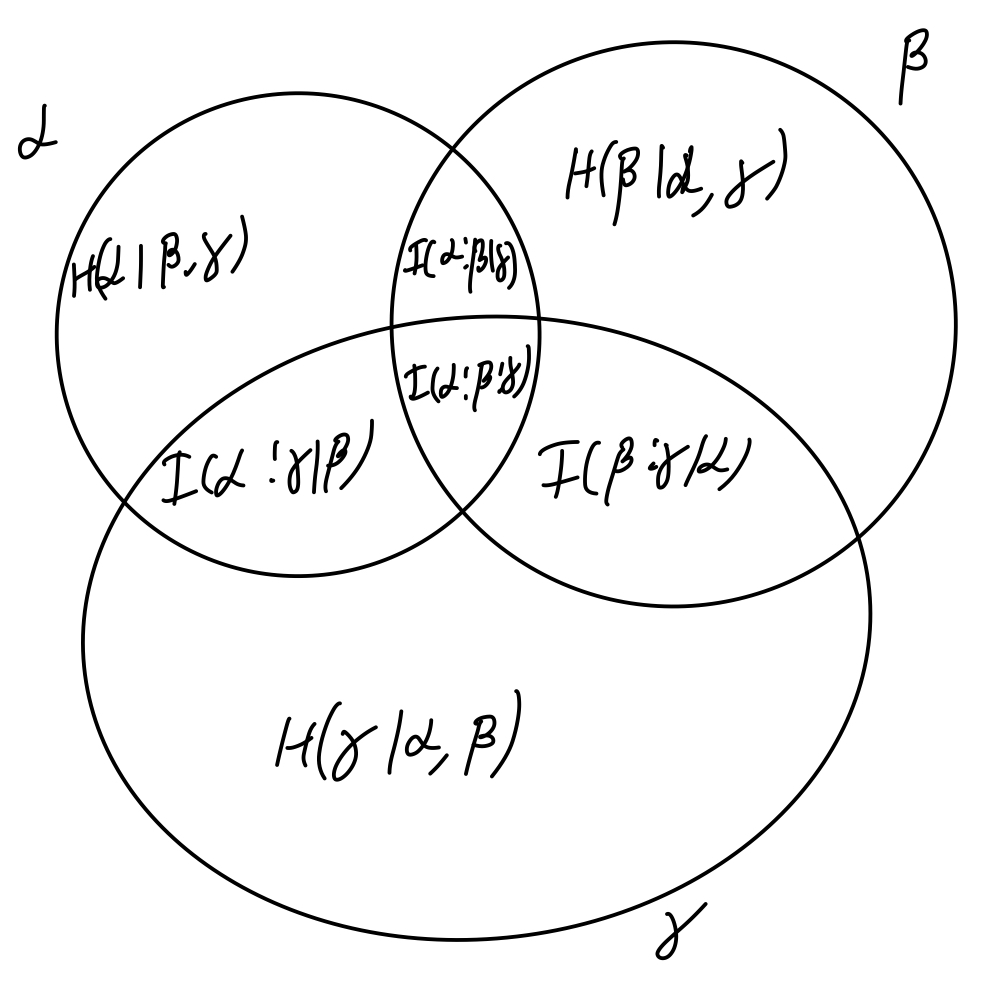
\includegraphics[width=0.3\textwidth]{IMG_FFE63C0B5F05-1}
	\caption{Circles for three variables.}
	\label{fig:IMG_FFE63C0B5F05-1}
\end{figure}

\begin{definition}
	The mutual information of three random variables $\alpha, \beta, \gamma$ is defined as
	\[
	I(\alpha : \beta : \gamma) = I(\alpha : \beta) - I(\alpha : \beta  \mid \gamma)
	.\] 
\end{definition}
\begin{statement}
	There are no other inequalities for triples.
\end{statement}
\begin{statement}
	The measure of profiles that cannot be expressed by any distribution is 0.
\end{statement}

\begin{statement}[Inequality for 5 random variables]
	For any random variables $a, b, x, y, z$:
	 \[
	I(a : b) \le  I(a : b  \mid x) + I(a : b  \mid  y) + I(x : y) + I(a : b  \mid z) + I(a : z  \mid b) + I(b : z  \mid  a)
	.\] 
\end{statement}

\begin{corollary}[Zhang, Yeung, 1998]
	An inequality for 4 random variables that cannot be expressed through the basic inequalities:
	\[
	I(a : b) \le  2 I(a : b  \mid x) + I(a : b  \mid  y) + I(x : y) + I(a : x  \mid b) + I(b : x  \mid  a)
	.\] 
\end{corollary}

\begin{statement}
	For 4 random variables, there are infinitely many inequalities that are independent of each other.
\end{statement}

The main idea was that for one variable we can realize any entropy.
For two variables we can realize any with properties.
With three almost any we can realize (with probability 0 we cannot).
With four and more nothing is known.

\subsection{Shearer's Lemma}
Remind a lemma that we had (in the homework).
\begin{lemma}
	\[
	2 H(\alpha, \beta, \gamma) \le  H(\alpha, \beta) + H(\alpha, \gamma) + H(\beta, \gamma)
	.\] 
\end{lemma}
So, on the right we have all the possible subsets of size two.
Generalized version:
\begin{theorem}[Shearer's Lemma]
	Let $X$ be a random variable distributed over $\{0, 1\}^{n}$.
	For any distribution $S$ on subsets of $[n]$, where $\Pr[i \in S] \geq \mu$ for each $i \in [n]$, it holds that
	 \[
		 \E_S[H(X_S)] \ge  \mu \cdot H(X).
	,\] where $X_S$ is a substring of  $X$ with indices in $S$. 
\end{theorem}
\begin{proof}
	In the homework.
	Hint: there is a common technique for proving it.
	We will use the an analogue of total probability formula.
	\[
		H(\alpha_1, \ldots, \alpha_n) = H(\alpha_1) + H(\alpha_2  \mid  \alpha_1) + H(\alpha_3  \mid \alpha_1, \alpha_2) + \ldots + H(\alpha_n  \mid \alpha_1, \ldots, \alpha_{n-1})
	.\] 
	Use this formula to prove the theorem.
	One needs to expand the inequality using formula and then do some manipulations.
\end{proof}
In fact, $X$ can be distributed over any set, but it would be easier to proof for now in  $\{0, 1\}^{n}$.
In lemma above $S$ is a uniform distribution over all subsets of $[3]$ of size $2$.
Then, $\Pr[i \in S] = \frac{2}{3}$.

\subsubsection{Counting Triangles in a Graph}


Consider an undirected graph $G = (V, E)$.
Let $l = |E|$.
And let  $t$ be a number of triangles.
\begin{lemma}
	\[
	t \le  \frac{(2l)^{3 / 2}}{6}
	.\] 
\end{lemma}
\begin{proof}
	Let the triplet of random variables $(\alpha, \beta, \gamma)$ be uniformly distributed over the vercies of the triangles (only triangles!).
	Let $X = (\alpha, \beta, \gamma)$.
	Then, $H(X) = H(\alpha, \beta, \gamma) = \log (6t)$ because it is uniform and each triangle counted six times.
	Consider the distribution $S$, uniform on subsets  $\{1, 2, 3\} $ of size 2.
	Then,
	\[
		\Pr[i \in S] = \frac{2}{3}
	.\] 
	Hence, By Shirer's Lemma:
	\[
		\E_S(H(X_S)) \ge  \frac{2}{3} \cdot \log (6t)
	.\] 
	I.e. there is $T \subset \{1, 2, 3\}  $ of size 2 such that $H(X_T) \geq \frac{2}{3} \log (6t)$.
	On the other hand, $X_T$ is a distribution over the edges of the graph (it can be nonuniform!), so  $\log (2l) \geq H(X_T)$.
	From that we get the desired bound.
\end{proof}

\subsection{Inequalities for Triplets}

\subsubsection{Warmup}

We will prove the following statement under various assuptions:
\[
H(a  \mid x) + H(a  \mid y) \le H(a)
.\] 

\begin{lemma} 
If $a, x, y$ are such that 
 \begin{align*}
	 \begin{cases}
	 	H(a  \mid x, y) = 0 \\
		I(x : y  \mid a) = 0.
	 \end{cases}
.\end{align*}
Then, $H(a  \mid  x) + H(a  \mid  y) \le  H(A)$.
\end{lemma}
\begin{proof}
	It is sufficient to prove that $I(x, y, a) \ge 0$.
	If it is negative, than $H(x, y) < 0$, contradiction.
	 \begin{figure}[htpb]
		\centering
		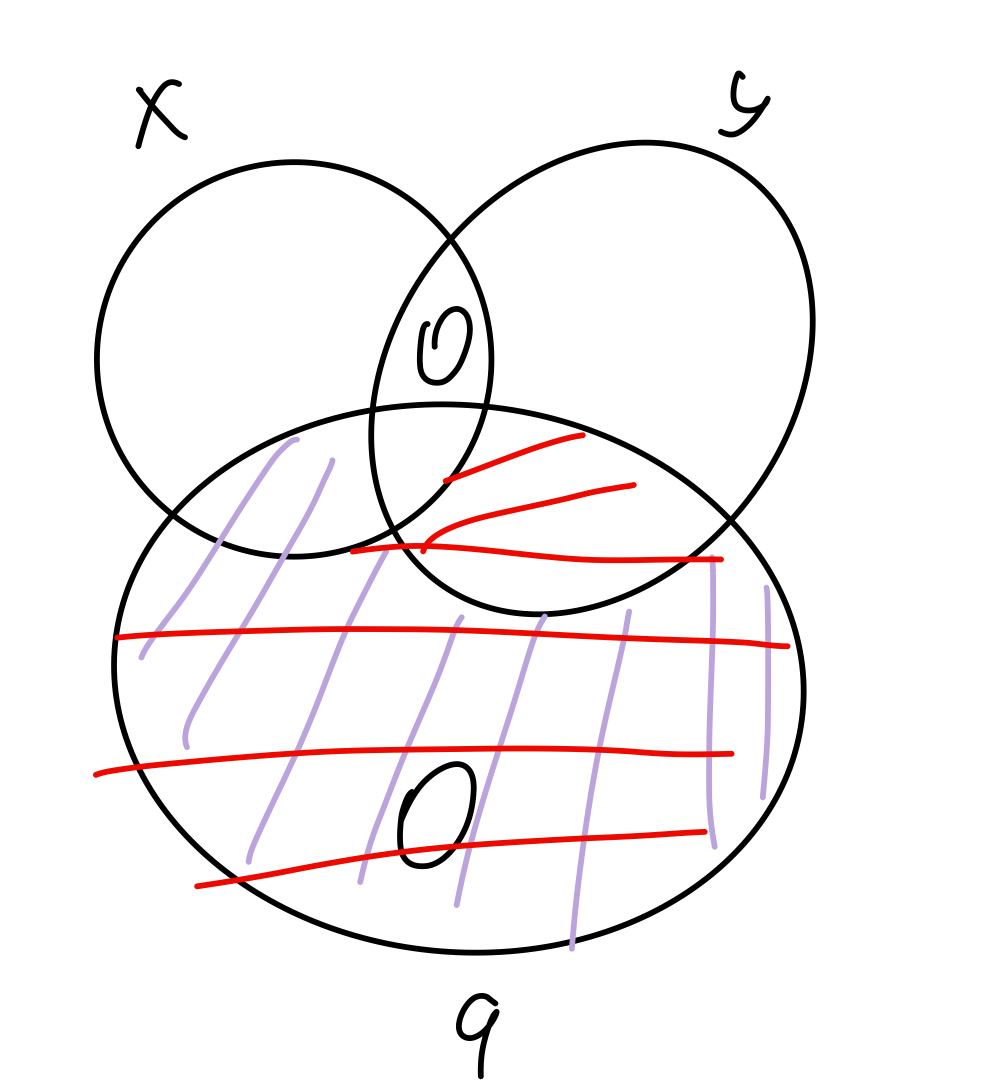
\includegraphics[width=0.3\textwidth]{IMG_C7FC1220B2AE-1}
		\caption{Structure of $a, x, y$.}
		\label{fig:IMG_C7FC1220B2AE-1}
	\end{figure}
	See \Cref{fig:IMG_C7FC1220B2AE-1}.
\end{proof}

\begin{theorem}
	If $a, x, y$ are such that $H(a \mid  x, y) = 0$ and
	 \begin{align*}
		\begin{cases}
			\Pr[a = A_i \land x = X_j] &> 0 \\
			\Pr[a = A_i \land y = Y_k] &> 0
		\end{cases} \implies \Pr[a = A_i \land x = X_j \land y = Y_k] > 0
	.\end{align*}
	For any $i, j, k$.
	Then,
	 \[
	H(a  \mid x) + H(a  \mid y) \le  H(a)
	.\] 
\end{theorem}
If $a = x \oplus y$, then

\begin{center}
\begin{tabular}{c|c|c}
	$a$ &  $x$ &  $y$ \\
	\hline
	0 & 0 & 0 \\
	1 & 0 & 1 \\
	1 & 1 & 0 \\
	0 & 1 & 1
\end{tabular}
\end{center}

So, both $(a = 1, x = 1), (a = 1, y = 1)$ are possible, but  $(a = 1, x = 1, y = 1)$ is not possible.
And the theorem statement is not satisfied.
\begin{proof}
	Since $H(a  \mid x, y)$, then $a = f(x, y)$ for some function  $f$. 
	By definition:
	\begin{align*}
		H(a, x, y) &= H(a) + H(x  \mid a) + \underbrace{H(y  \mid a, x)}_{H(y  \mid a) - I(x : y  \mid a)}.
	\end{align*}
	Since we know nothing about $I(x : y  \mid a)$, we will construct new variables.
	Define $a' \sim a$.
	Then, let  $x' \sim x$ and  $x'  \mid a'$ has the same distribution as $x | a$.
	And the same for $y'$, i.e. $y' \sim y$ and $y'  \mid a'$ has the same distribution as $y  \mid a$.
	But also we require that $x'$ and  $y'$ are independent (if we think of probabilities as some matrix with the probability of each event, then we can construct those easily).
	Hence,
	 \[
		 \Pr[x' = X_i \land y' = Y_k] = \Pr[x' = X_i] \cdot \Pr[y' = Y_k]
	.\] 
	The idea is that now,
	\begin{align*}
		H(a', x', y') &= H(a') + H(x'  \mid a') + H(y'  \mid a') - \underbrace{I(x' : y'  \mid a')}_{0}.
	\end{align*}
	Also,
	\begin{align}
		H(a', x', y') &\leq H(a'  \mid x', y') + H(x') + H(y') &\implies \nonumber \\
		H(a') + H(x'  \mid a') + H(y'  \mid a') &\leq H(a'  \mid  x', y') + H(x') + H(y') \label{eq:1}
	.\end{align}
	One can see that $H(a'  \mid x', y')$.
	Assume that it is not true and for some pair $X_{j}, Y_K$ we have that $a$ could be  $A_1$ or $A_2$, but we have a contradiction with the statement, since
	\begin{align*}
		\begin{cases}
			\Pr[x' = X_j' \land y' = Y_k \land a' = A_1] > 0, \\
			\Pr[x' = X_j' \land y' = Y_k \land a' = A_2] > 0.
		\end{cases}
	\end{align*},
	but
	\begin{align*}
		0 < \Pr[x' = X_j \land y' = Y_k  \mid a' = A_i] = \Pr[x' = X_j  \mid a' = A_i] \cdot \Pr[y' = Y_k  \mid a' = A_i]
	.\end{align*}
	Hence, we have a contradiction with the statement.
	Hence, rewriting \eqref{eq:1} we get:
	\begin{align*}
		H(a') + H(x'  \mid a') + H(y'  \mid a') &\leq H(x') + H(y') &\implies \\
		H(a) + H(x  \mid a) + H(y  \mid a) &\leq H(x) + H(y) &\implies \\
		\underbrace{2H(a) + H(x  \mid a) + H(y  \mid a)}_{\geq H(a  \mid x) + H(a  \mid y)} &\leq H(a) + H(x) + H(y) &\implies \\
		H(a  \mid x) + H(a  \mid y) &\leq H(a)
	.&\qedhere\end{align*}
\end{proof}

\begin{example}
	We have a rectangular sheet divided into rectangles.
	It is not necessary for the cut lines to extend from edge to edge (some cuts may be inside).
	It is known that any horizontal line intersects at least $n$ rectangles and any vertical line intersects at least $m$ rectangles.
	Prove that in this partition, there are at least  $mn$ rectangles.
 \end{example}
 \begin{proof}
	 See \Cref{fig:IMG_A0ED442FB3AB-1}.
	 \begin{figure}[htpb]
	 	\centering
	 	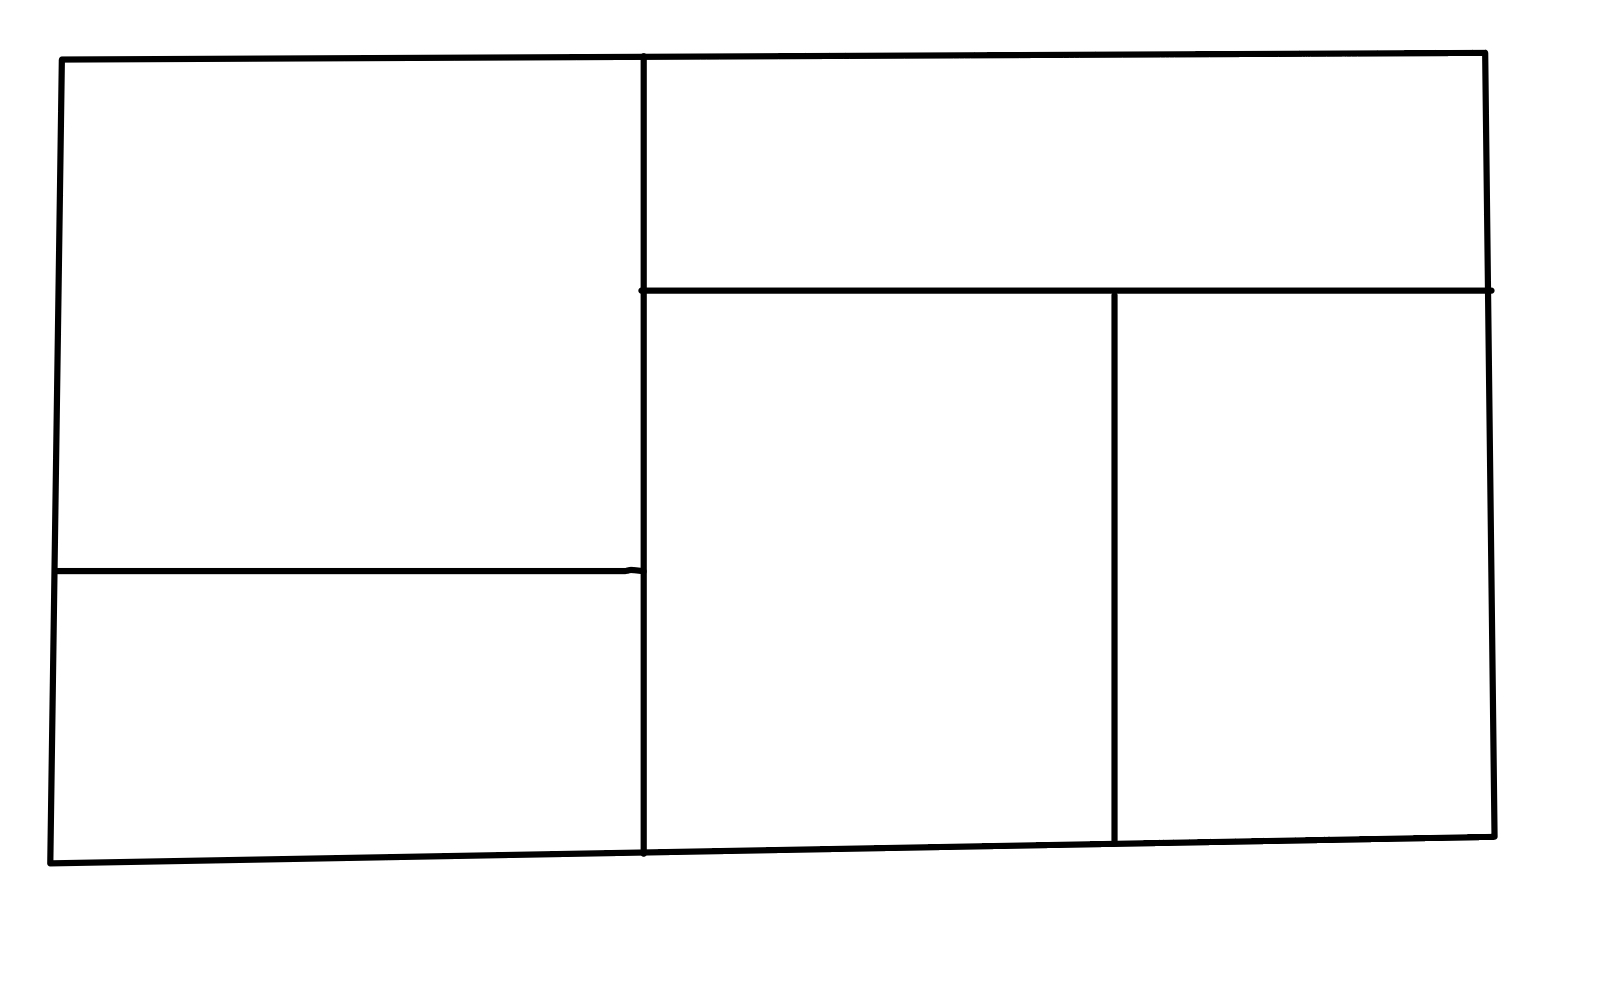
\includegraphics[width=0.3\textwidth]{IMG_A0ED442FB3AB-1}
	 	\caption{Division of the rectangles.}
	 	\label{fig:IMG_A0ED442FB3AB-1}
	 \end{figure}

	 Let $x, y$ be some coordinates (uniform distribution).
	 Then,  $a$ is a rectangle that contains $(x, y)$.
	 Then,  $a = f(x, y)$.
	 We know that  $H(x) \geq \log m$ and  $H(y) \geq \log n$.
	 And also if I can be in a rectangle  $A_I$ with coordinate $X_j$ and  $Y_k$  
	 Hence, using our theorem we know that:
	 \[
	 H(a  \mid x) + H(a  \mid y) \le  H(a)
	 .\] 
	 And $H(a  \mid x) \geq \log m, H(a  \mid y) \geq m$ and $H(a)$ is a log of number of rectangles.
 \end{proof}
